\documentclass[a4paper]{article}
\usepackage[utf8]{inputenc}
\usepackage[T1]{fontenc}
\usepackage[slovene]{babel}
\usepackage{lmodern} 
\usepackage{hyperref}
\usepackage{blindtext}
\usepackage{amsmath}  % razna okolja za poravnane enačbe ipd.
\usepackage{amsthm}   % definicije okolij za izreke, definicije, ...
\usepackage{amssymb}  % dodatni matematični simboli
\usepackage{listings} % okolje za Python kodo
\usepackage{xcolor}   % okolje za barve (za kodo)
\usepackage{graphicx} % okolje za slike

\definecolor{codegreen}{rgb}{0,0.6,0}
\definecolor{codegray}{rgb}{0.5,0.5,0.5}
\definecolor{codepurple}{rgb}{0.58,0,0.82}

\lstdefinestyle{mystyle}{   
    commentstyle=\color{codegreen},
    keywordstyle=\color{magenta},
    numberstyle=\tiny\color{codegray},
    stringstyle=\color{codepurple},
    basicstyle=\ttfamily\footnotesize,
    breakatwhitespace=false,         
    breaklines=true,                 
    captionpos=b,                    
    keepspaces=true,                 
    numbers=left,                    
    numbersep=5pt,                  
    showspaces=false,                
    showstringspaces=false,
    showtabs=false,                  
    tabsize=2
}
\lstset{language=Python, style=mystyle}

\title{\textit{Grid-peeling}}
\author{Gašper Pust, Mitja Mandić}
\begin{document}

\begin{titlepage}
 \maketitle
\end{titlepage}

\section{Predstavitev problema}
V projektu si bova podrobneje ogledala konveksne ovojnice $m \times n$ mreže. Konveksna ovojnica množice je najmanjša konveksna množica, ki vsebuje dano množico točk.
Najlažje si jo predstavljamo tako, kot da bi okoli elementov množice napeli elastiko - kar elastika obkroži, je konveksna ovojnica. Lupljenje konveksnih ovojnic mreže,
(angl. \textit{grid-peeling}) je proces, ko iz mreže iterativno odstranjujemo konveksne ovojnice. S simboli lahko to zapišemo takole:
$ P_{0} = G_{m,n} = \{0,\ldots, m-1\} \times \{0, \ldots, n-1\}$. Naj bo $C_{i} = \mathcal{C}\mathcal{H}(P_{i-1}) \text{ za } i = 1, \ldots$. $V_{i}$ naj bo množica vozlišč $C_{i}$
- kot vozlišče razumemo točko, ki je na vogalu mreže (torej za katero bi zataknili elastiko). Naj bo sedaj $P_{i} = P_{i-1} \setminus V_{i}$. Začnemo torej z $n \times m$ mrežo 
in iterativno lupimo konveksne ovojnice, dokler ne odstranimo vseh točk.

V projektni nalogi bova s pomočjo simulacij opazovala v literaturi navedene številke za $n \times n$ mrežo - teorija napoveduje $\theta(n ^ \frac{4}{3})$ ovojnic.
Za $m \times n$ mrežo v literaturi ni navedenih podatkov, zanimala pa naju bo morebitna povezava. Simulacije bova izvedla tudi za točke na neenakomerni mreži.

Po izvedenem eksperimentalnem delu, bova rezultate analizirala in jih primerjala z rezultati iz literature. Zanimalo naju bo, kako drugačno je število ovojnic na $m \times n$
mreži v primerjavi s simetrično.

\section{Orodja in algoritmi}
Za uporabo algoritmov v Pythonu sva najprej definirala razred Točka, v katerem sva skonstruirala vsa potrebna orodja in funkcije za uporabo algoritmov za iskanje konveksnih ovojnic.

\begin{lstlisting}
class Tocka:
    def __init__(self, x, y):
        self.x = x
        self.y = y

    def kot_med_dvema(self, other):
        if self.x != other.x:
            return (self.y - other.y) / (self.x - other.x)
        else:
            return 90

    def vektorski_produkt(self, other): 
        return self.x * other.y - self.y * other.x

    def razlika(self, other):
    	return Tocka(self.x - other.x, self.y - other.y)

    def razdalja(self, other):
        return (self.x - other.x) ** 2 + (self.y - other.y) ** 2

    def __str__(self):
        return '(' + str(self.x) + ', ' + str(self.y) + ')'

    def __repr__(self):
        return 'T(' + str(self.x) + ', ' + str(self.y) + ')'

def smer_razlike(p,q,r):
    return p.razlika(q).vektorski_produkt(r.razlika(q))

def enakomerna_mreza(m,n):
    return [Tocka(i,j) for i in range(m) for j in range(n)]

def naredi_potencno(m, n):
    return [Tocka(2**i,2**j) for i in range(m) for j in range(n)]

def kvazi_cantor_mreza(n):
    sez = [0,3]
    for i in range(1,n):
        nasl_dol = sez[0] - 3 ** i
        nasl_gor = sez[-1] + 3 ** i
        sez.append(nasl_gor)
        sez = [nasl_dol] + sez
    return [Tocka(i,j) for i in sez for j in sez]
\end{lstlisting}

Zgornje funkcije bova uporabila v dveh različnih algoritmih za iskanje konveksnih ovojnic, in sicer v Jarvisovem obhodu in Grahamovemu pregledu.
Oba algoritma sprejmeta seznam točk in mu priredita konveksno ovojnico, a to storita na drugačen način.
Seznam točk ustvarijo zadnje tri funkcije zgoraj, pri čemer prva sestavi enakomerno mrežo točk $(i, j),$~druga ustvari mrežo točk oblike $(2^i, 2^j),$~tretja pa oblikuje mrežo, ki
jo začnemo graditi na sredini in ima na $i$-tem koraku dolžino vsake od stranic $3^i,$~v množico pa na vsakem koraku dodamo kotne točke te mreže. Ker je vsaka prejšnja stranica
ravno srednja tretjina naslednje, sva mrežo poimenovala ,,kvazi-Cantorjeva mreža.''

\subsection{Jarvisov obhod}
Jarvisov obhod (angl. \textit{Jarvis March}) ali algoritem zavijanja darila je postopek, ki dani množici točk poišče konveksno ovojnico v eni ali več dimenzijah (osredotočili se 
bomo na dve dimenziji). Algoritem se imenuje po R.A. Jarvisu, ki ga je objavil leta 1973. Časovna zahtevnost algoritma je $O(nh),$~kjer $n$~predstavlja število vseh točk, $h$~pa 
število točk, ki ležijo na konveksni ovojnici. V najslabšem primeru, ko so vse podane točke tudi elementi konveksne ovojnice, torej v primeru $h = n,$~je njegova časovna zahtevnost 
$O(n^2)$. Jarvisov obhod se največkrat uporablja za majhne $n$~ali pa v primeru, ko pričakujemo, da bo $h$~zelo majhen glede na $n$.

\begin{lstlisting}
def jarvis_march(seznam):
    zacetna_tocka =  min(seznam, key = lambda tocka: tocka.x)
    indeks = seznam.index(zacetna_tocka) 
    l = indeks
    rezultat = []
    rezultat.append(zacetna_tocka)
    while (True):
        q = (l + 1) % len(seznam)      
        for i in range(len(seznam)):
            if i == l:
                continue
            d = smer_razlike(seznam[l], seznam[i], seznam[q])
            if d > 0 or (d == 0 and seznam[i].razdalja(seznam[l]) > seznam[q].razdalja(seznam[l])):
                q = i
        l = q
        if l == indeks:
            break    
        rezultat.append(seznam[q])
    return rezultat
\end{lstlisting}

Algoritem najprej poišče najbolj levo točko (2. vrstica kode). Potem ustvari prazen seznam, v katerega postopoma dodaja točke, ki jih obišče. 

Vanj najprej doda začetno točko, označimo jo z $l$, nato izberemo poljubno točko, ki jo označimo s $q$ (8. vrstica kode - tu je q točka izbrana tako, da je zagotovo v seznamu, 
lahko bi izbrali katerokoli razen začetne). Potem se začne iteracija, točke v iteraciji označimo z $i$. Če kot $(l,i,q)$ predstavlja ovinek v desno, $q$ in $i$ zamenjamo,
če je ta kot ovinek v levo nadaljujemo brez sprememb, če pa so točke $p,q\text{ter~}i$ kolinearne, izmed $q \text{in}i$ izberemo tisto, ki ima večjo $x$ koordinato
(je dlje od začetne točke). Ko tako pridemo do konca in pregledamo vse točke, smo konveksno ovojnico našli in jo algoritem vrne kot seznam točk. 

Opisan postopek se v zgornji kodi odvije od 7. do 15. vrstice. Funkcija \texttt{ smer\textunderscore razlike } izračuna kot med vektorji 
(oziroma natančneje, izračuna vektorski produkt vektorjev $(l - i)\times(q - i)$). Če je ta vrednost pozitivna (imamo ovinek v desno) oziroma 0 in je $i$ dlje od začetne točke kot $q$, zamenjamo $q$ in $i$. 

Na koncu preverimo, če smo prišli nazaj v začetno točko $l.$ V tem primeru algoritem ustavimo, ali pa postopek ponovimo z novo začetno točko. To je tista, ki smo jo
v prejšnji ponovitvi zanke dodali v ovojnico.

\subsection{Grahamov pregled}
Alternativa prejšnjemu algoritmu je tako imenovani Grahamov pregled (angl. \textit{Graham's scan}). Algoritem se imenuje po Ronaldu Grahamu, ki ga je objavil leta 1972. 
V primerjavi z Jarvisovim obhodom je Grahamov pregled hitrejši, saj ima časovno zahtevnost $O(n \log n)$.

\begin{lstlisting}
def uredi_po_kotu(seznam):
    prvi = min(seznam, key = lambda tocka: (tocka.x, tocka.y))
    return [prvi] + sorted(seznam[1:], key=lambda x: prvi.kot_med_dvema(x))

def graham_scan(seznam):
    urejene_tocke = uredi_po_kotu(seznam)
    ovojnica = []
    for tocka in urejene_tocke:
        while len(ovojnica) > 1 and smer_razlike(ovojnica[-2], ovojnica[-1], tocka) >= 0:           
            ovojnica.pop()
        ovojnica.append(tocka)
    return ovojnica
\end{lstlisting}

Najprej definiramo funkcijo, ki seznam uredi po naraščajočem kotu med točkama, glede na $x$-os. Za urejanje uporabimo kar vgrajeno Pythonovo funkcijo \texttt{sorted},
ki bazira na \textit{timsort} algoritmu, ki ima časovno zahtevnost $O(n \log n).$ Dodali smo le še funkcijo, ki računa kot med dvema točkama, kar pa se zgodi v linearnem času.

Algoritem najprej točke uredi po kotu in ustvari prazen seznam (kopico), 
v katerega bo dodajal točke, ki so v konveksni ovojnici.

Najprej v kopico dodamo prvi dve točki iz urejenega seznama, ti bosta zagotovo tudi v konveksni ovojnici.
Če je v kopici več kot ena točka, vzame zadnji dve točki v ovojnici in prvo iz urejenega seznama ter preveri kot med njimi. Če torej označimo zadnji dve točki iz kopice z $x$ in $y$ ter točko,
ki je prva v seznamu z $i$, izračunamo vektorski produkt $(x-y)\times(i-y)$. 
Če je pozitiven (kot z vrhom v $y$ in krakoma skozi $x$ ter $i$ predstavlja ovinek v desno), točko izloči, 
sicer pa jo doda na vrh kopice (v našem primeru na konec seznama). Ko pregleda vse urejene točke, se ustavi. 
V zanki moramo le enkrat pregledati vse točke, in ker se vse zgoraj opisano računanje izvaja v linearnem času, je zahtevnost tega dela $O(n)$ (kar pa je manj od zahtevnosti urejanja,
torej je to zgornja meja za zahtevnost algoritma).

\section{Algoritem za lupljenje konveksnih ovojnic}
S pomočjo zgornjih algoritmov sedaj lahko izpeljemo algoritem za lupljenje konveksnih ovojnic. Glede na vrsto iskanja konveksnih ovojnic, torej po Jarvisovem ali 
Grahamovem načinu, ločimo dva algoritma, ki pa se razlikujeta le v koraku, v katerem iščemo konveksno ovojnico.

\begin{lstlisting}
def grid_peel_graham(mreza): #oz. grid_peel_jarvis(mreza)
    start = time.time()
    ovojnice = {}
    i = 0
    while mreza or len(mreza) > 1:
        ch = graham_scan(mreza) #oz. ch = jarvis_march(mreza)
        nova = [x for x in mreza if x not in ch]
        mreza = nova
        ovojnice[i] = ch
        i += 1
    casovna_zahtevnost = time.time() - start 
    return i, ovojnice, casovna_zahtevnost
\end{lstlisting}

V obeh primerih algoritem najprej označi začetni čas in ustvari prazno množico, v katero bo kasneje shranjeval konveksne ovojnice. Dokler seznam točk ni prazen, algoritem na vsakem koraku 
poišče konveksno ovojnico (6. vrstica kode, tu se algoritma razlikujeta) in iz seznama mrežnih točk odstrani vse točke, ki so v konveksni ovojnici. Točke v konveksni ovojnici, dobljeni na 
$i$-tem koraku, doda v množico konveksnih ovojnic kot $i$-ti element in števec poveča za 1. To je del kode od 5. do 10. vrstice (v obeh algoritmih). Preden vrne rezultat, algoritem še enkrat 
izmeri čas, ki mu odšteje začetnega in razlika predstavlja čas potreben za izvedbo algoritma. Kot rezultat algoritma vrneta število korakov do prazne mreže, množico konveksnih ovojnic in pa 
potreben čas za izvedbo algoritma. S pomočjo množice konveksnih ovojnic lahko postopek lupljenja $m \times n$~mreže tudi narišemo.

\subsection{Prikaz rezultatov na primerih}
Za boljšo predstavo, kako algoritem deluje, sva postopek lupljenja konveksnih ovojnic prikazala na nekaj primerih. Prvi, ki je prikazan na sliki \ref{fig:11x11}, je postopek lupljenja 
navadne mreže velikosti $11 \times 11,$~drugi, prikazan na sliki \ref{fig:15x10}, pa je psotopek lupljenja navadne mreže velikosti $15 \times 10$. 

\begin{figure}[!h]
	\centering
	\caption{Postopek lupljenja ovojnic enakomerne $11 \times 11$ mreže}
	\label{fig:11x11}
	\vspace{2mm}
	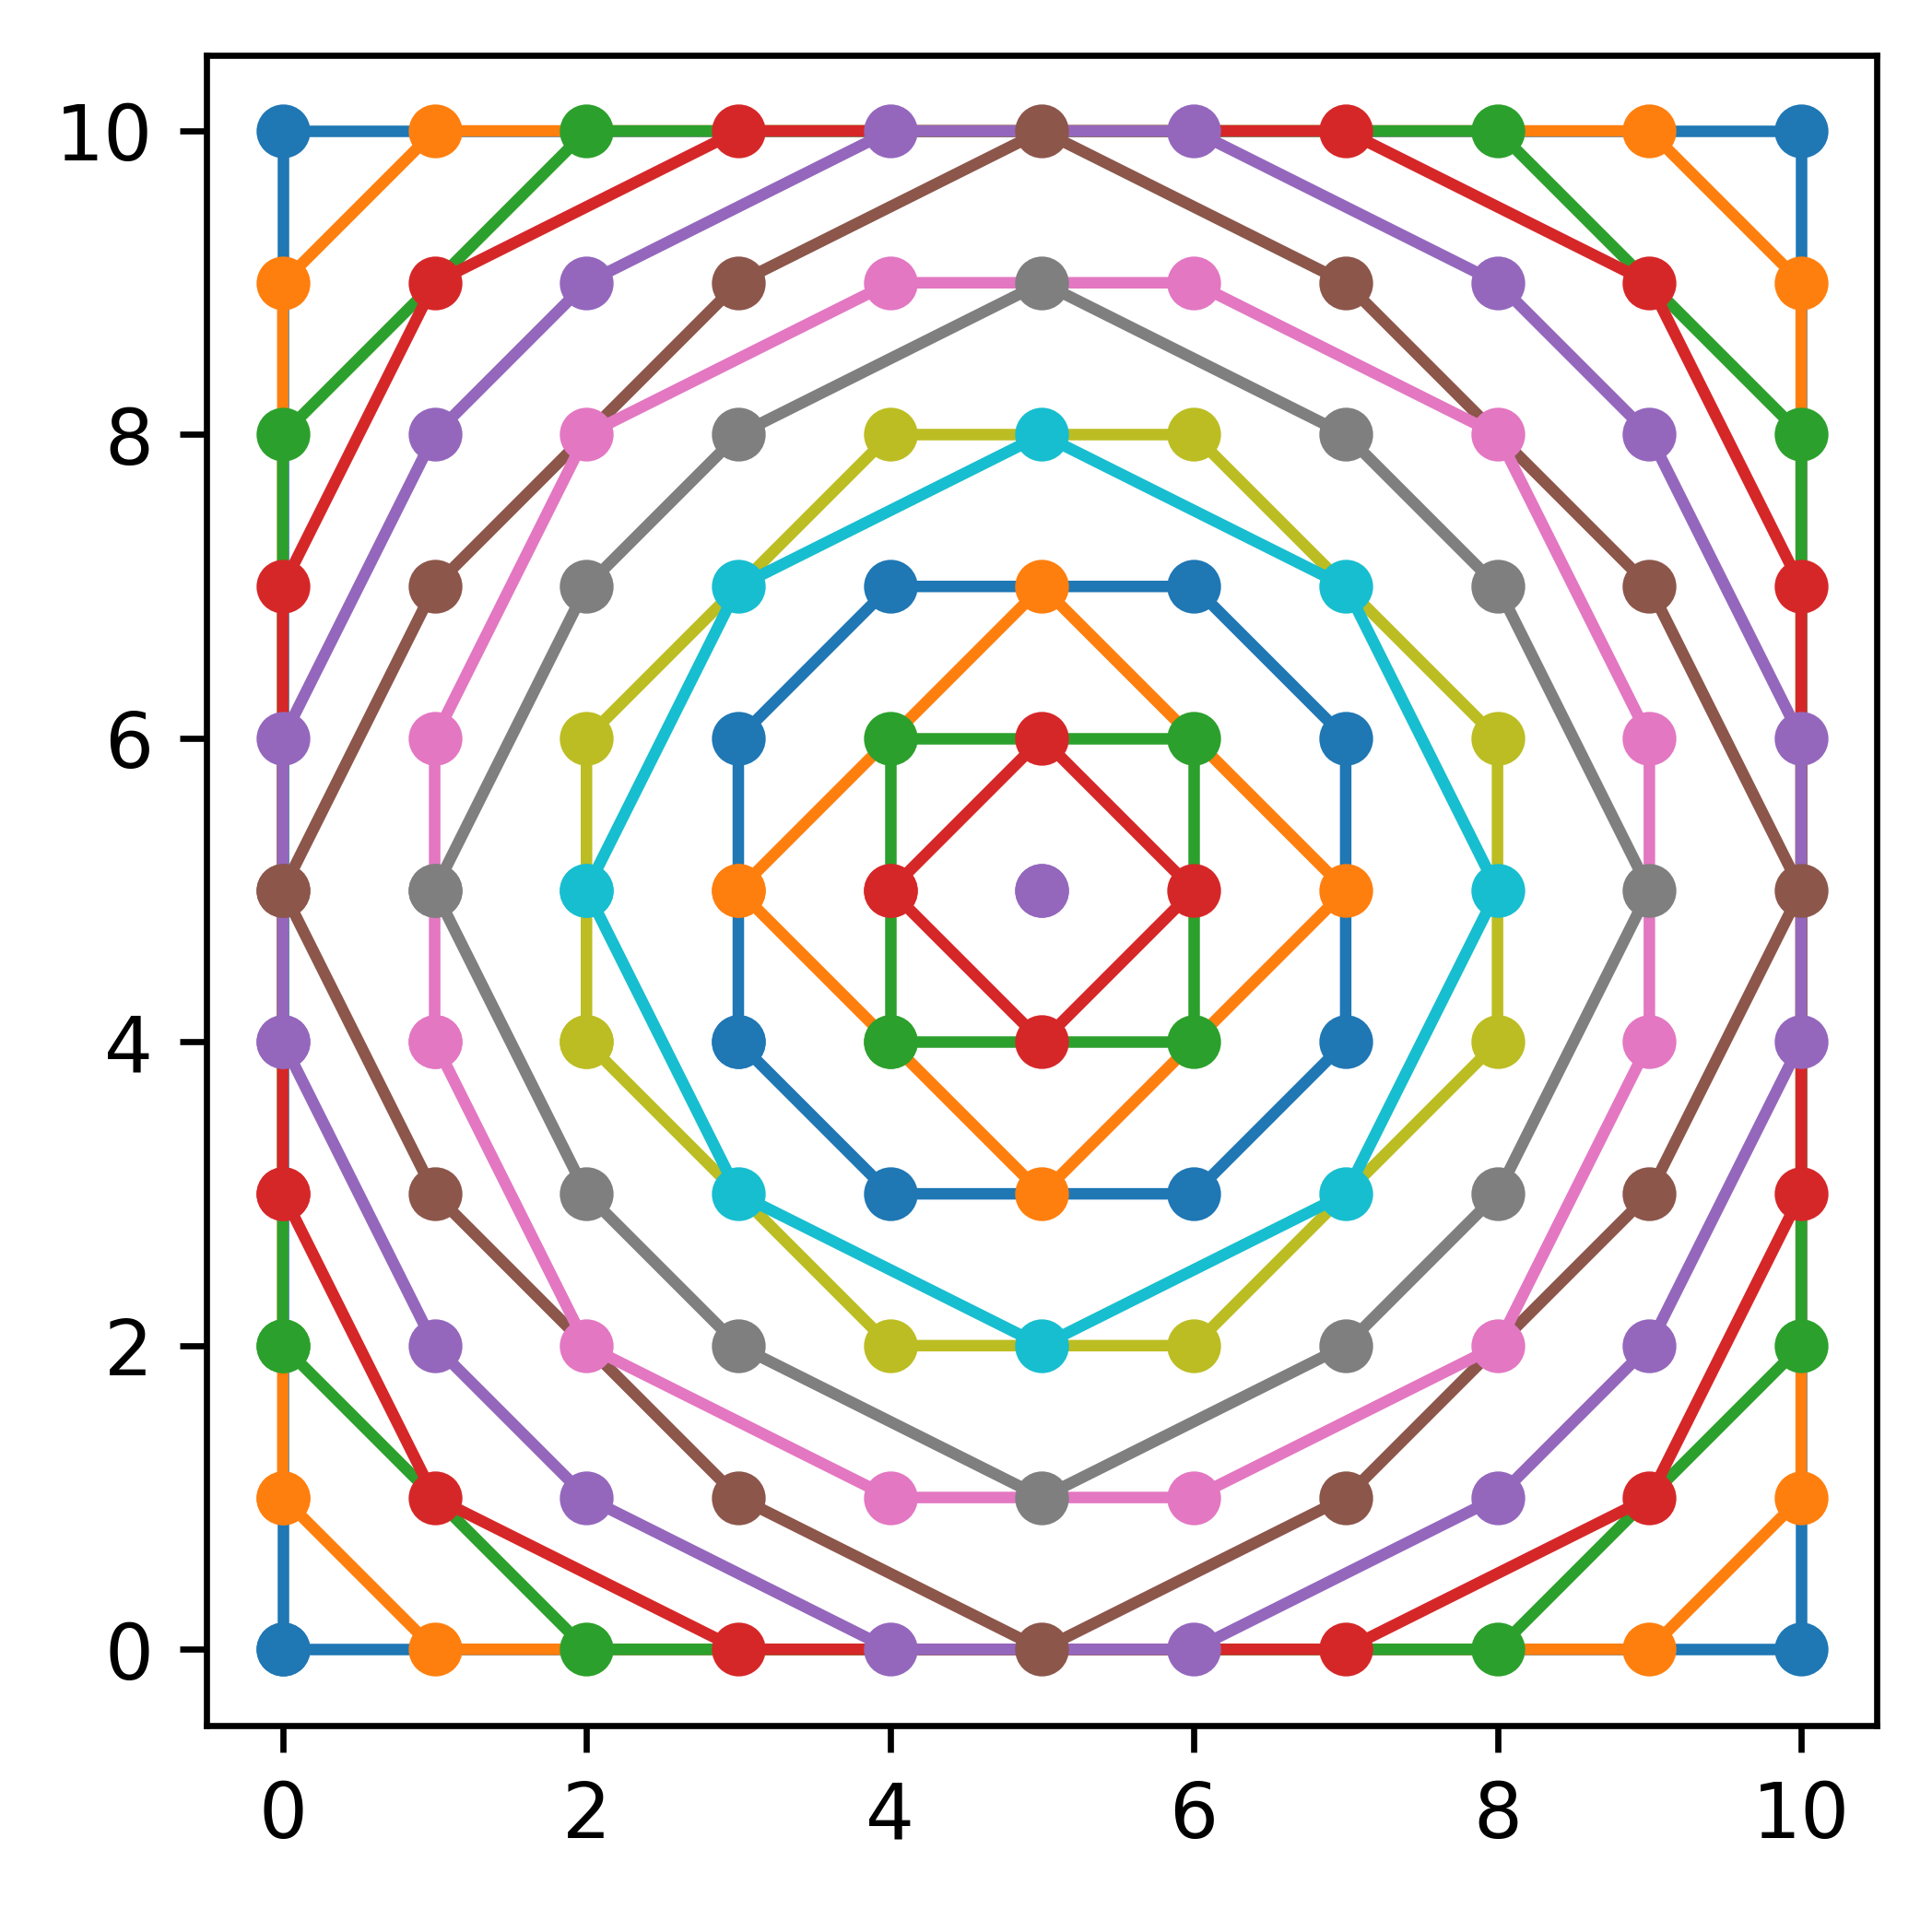
\includegraphics[scale=0.6]{slike/11x11_enakomerna.png}
\end{figure}

\begin{figure}[!h]
	\centering
	\caption{Postopek lupljenja ovojnic enakomerne $15 \times 10$ mreže}
	\label{fig:15x10}
	\vspace{2mm}
	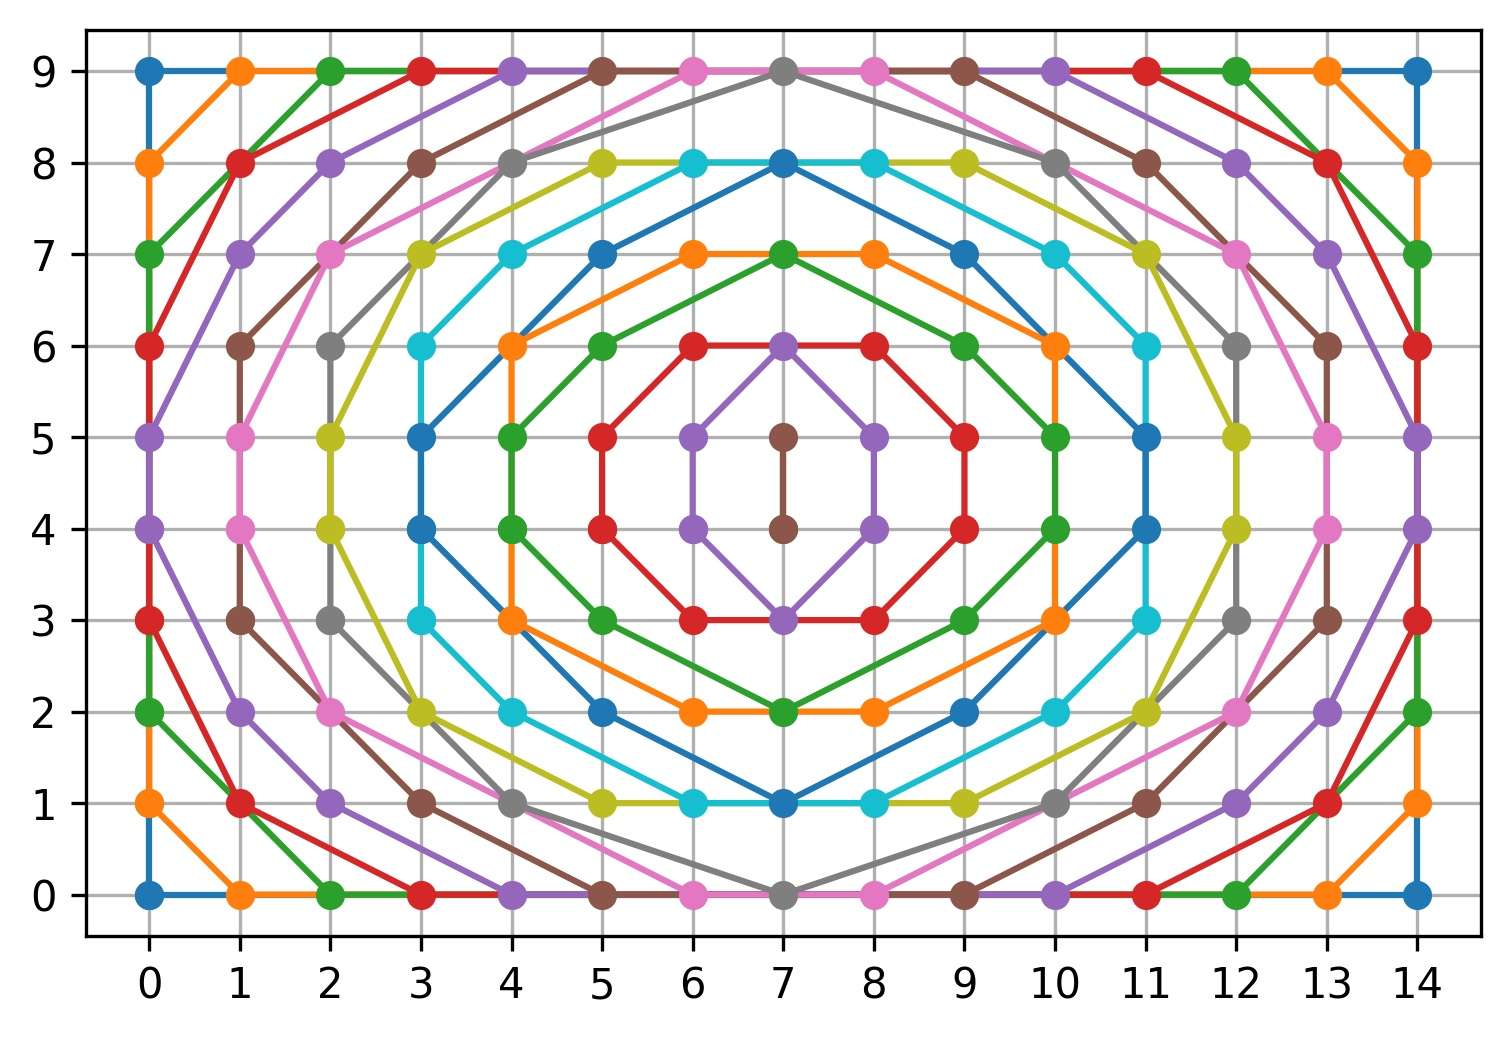
\includegraphics[scale=0.6]{slike/15x10_enakomerna.jpg}
\end{figure}

\newpage
Na sliki \ref{fig:5x5} je prikazan postopek na potenčni mreži velikosti $5 \times 5$, na sliki \ref{fig:cantor} pa postopek na Cantorjevi mreži velikosti $4 \times 4$.

\begin{figure}[!h]
	\centering
	\caption{Postopek lupljenja ovojnic potenčne $5 \times 5$ mreže}
	\label{fig:5x5}
	\vspace{2mm}
	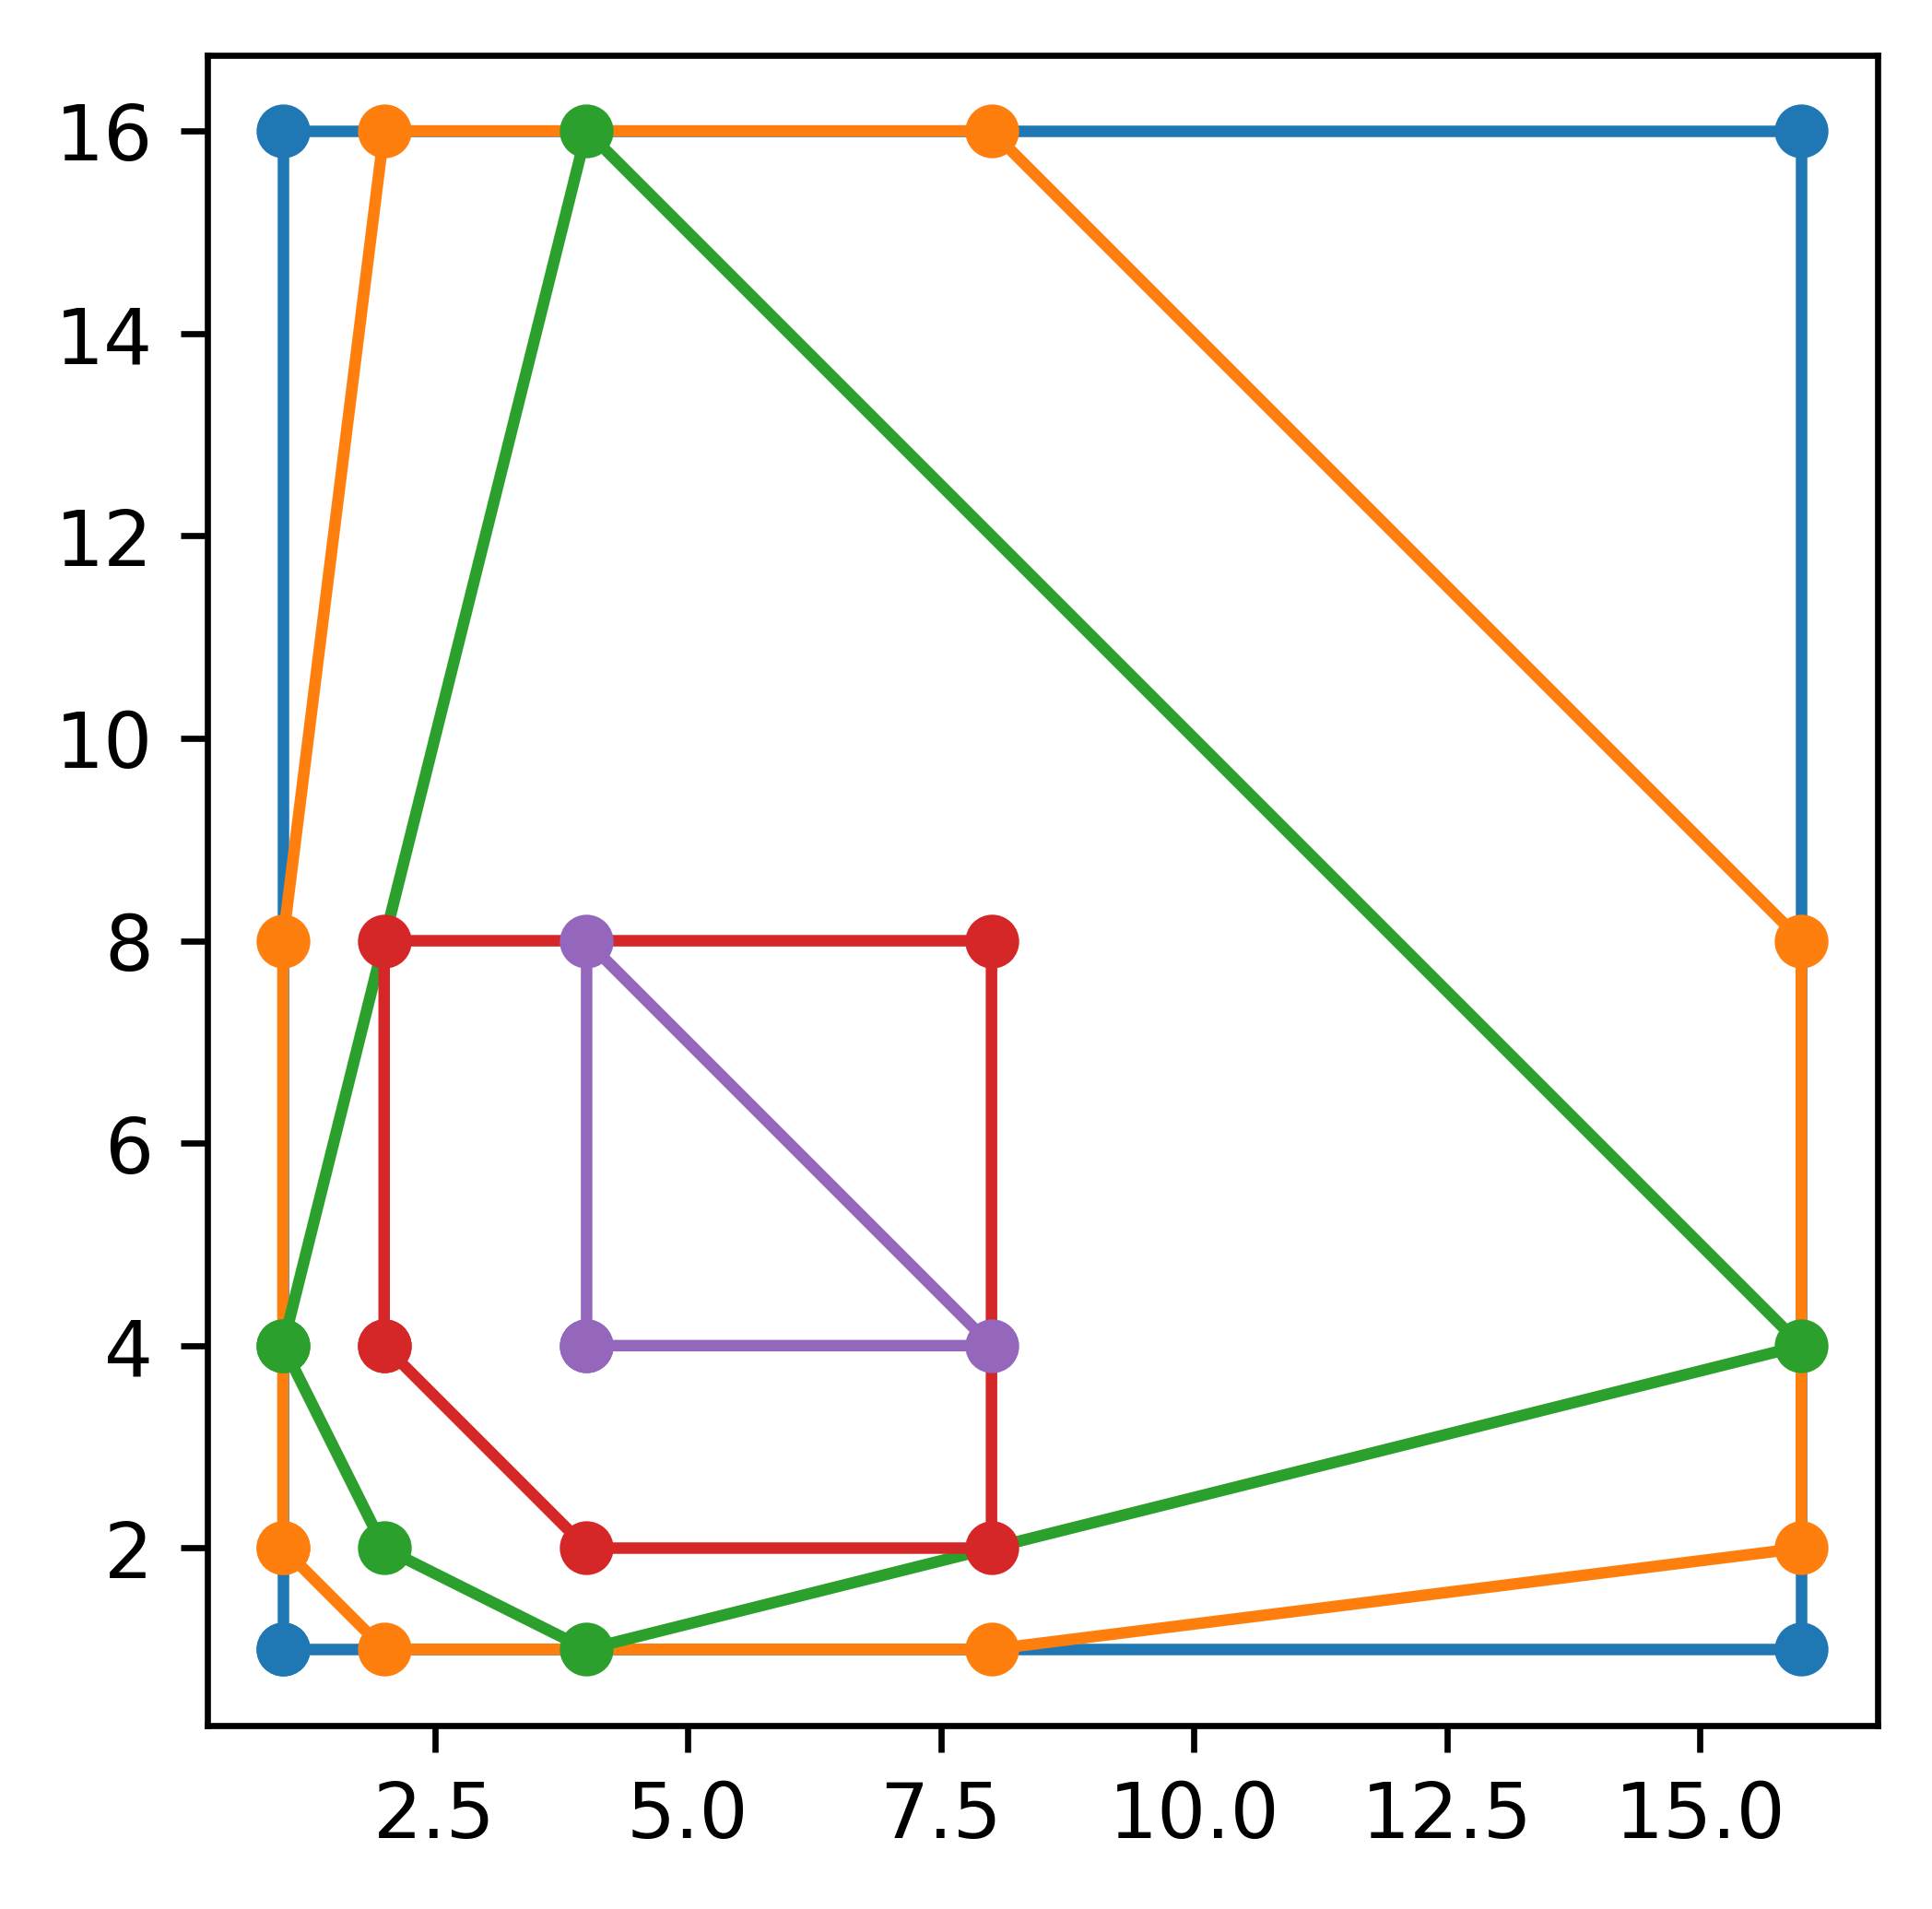
\includegraphics[scale=0.6]{slike/5x5_potencna.png}
\end{figure}

\begin{figure}[!h]
	\centering
	\caption{Postopek lupljenja ovojnic Cantorjeve $8 \times 8$~mreže}
	\label{fig:cantor}
	\vspace{2mm}
	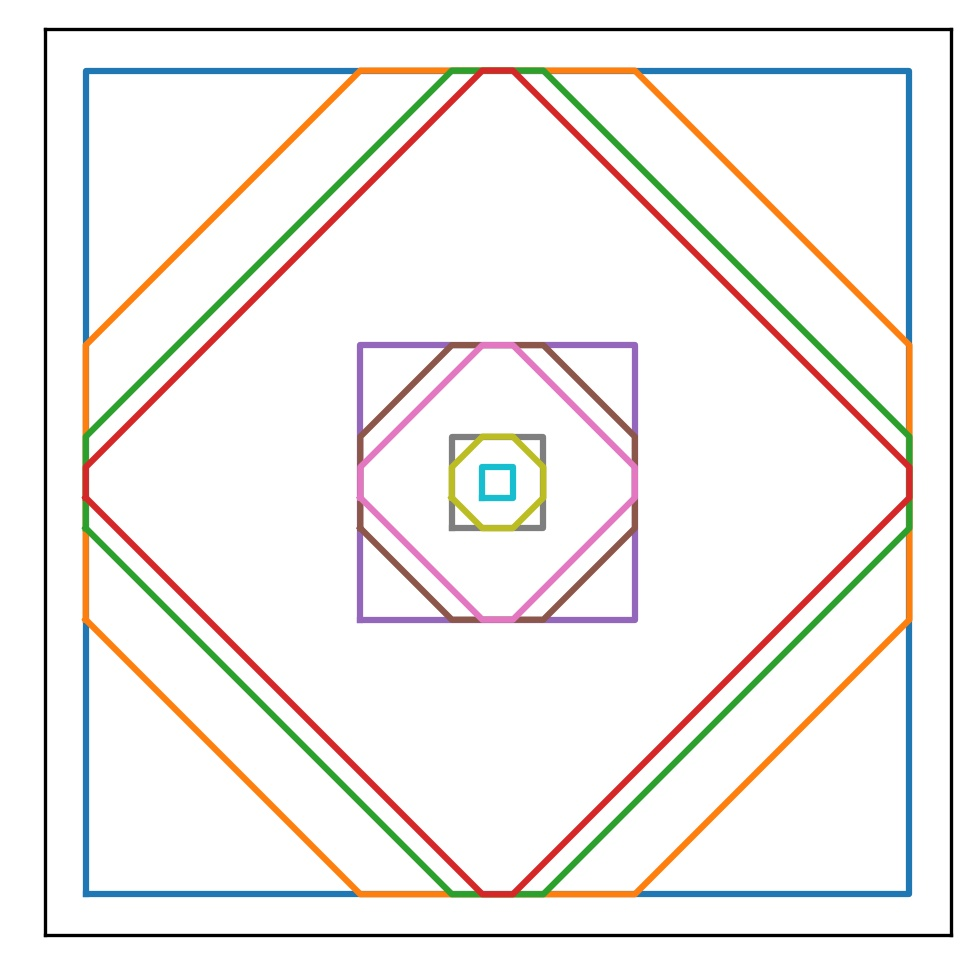
\includegraphics[scale=0.6]{slike/kvazi_cantor.jpg}
\end{figure}

\subsection{Časovna zahtevnost algoritma}
Najprej bova prikazala časovno primerjavo med Jarvisovim obhodom in Grahamovim pregledom. Glede na izbrani algoritem za iskanje konveksnih ovojnic se čas izvajanja algoritma za lupljenje
lahko zelo razlikuje, kar je jasno razvidno iz slike \ref{fig:cas}. Tu sva prikazala samo primer $n \times n$~mreže, vendar pa je za $m \times n$~mreže rezultat podoben. Absolutni
čas izvajanja algoritma je seveda odvisen od številnih dejavnikov (zmogljivost računalnika, koliko procesov se izvaja v ozadju, \ldots), vendar se jasno vidi
večjo učinkovitost Grahamovega pregleda.

\begin{figure}[!h]
	\centering
	\caption{Čas izvedbe algoritma lupljenja konveksnih ovojnic $n \times n$ mreže v odvisnosti od $n$}
	\label{fig:cas}
	\vspace{2mm}
	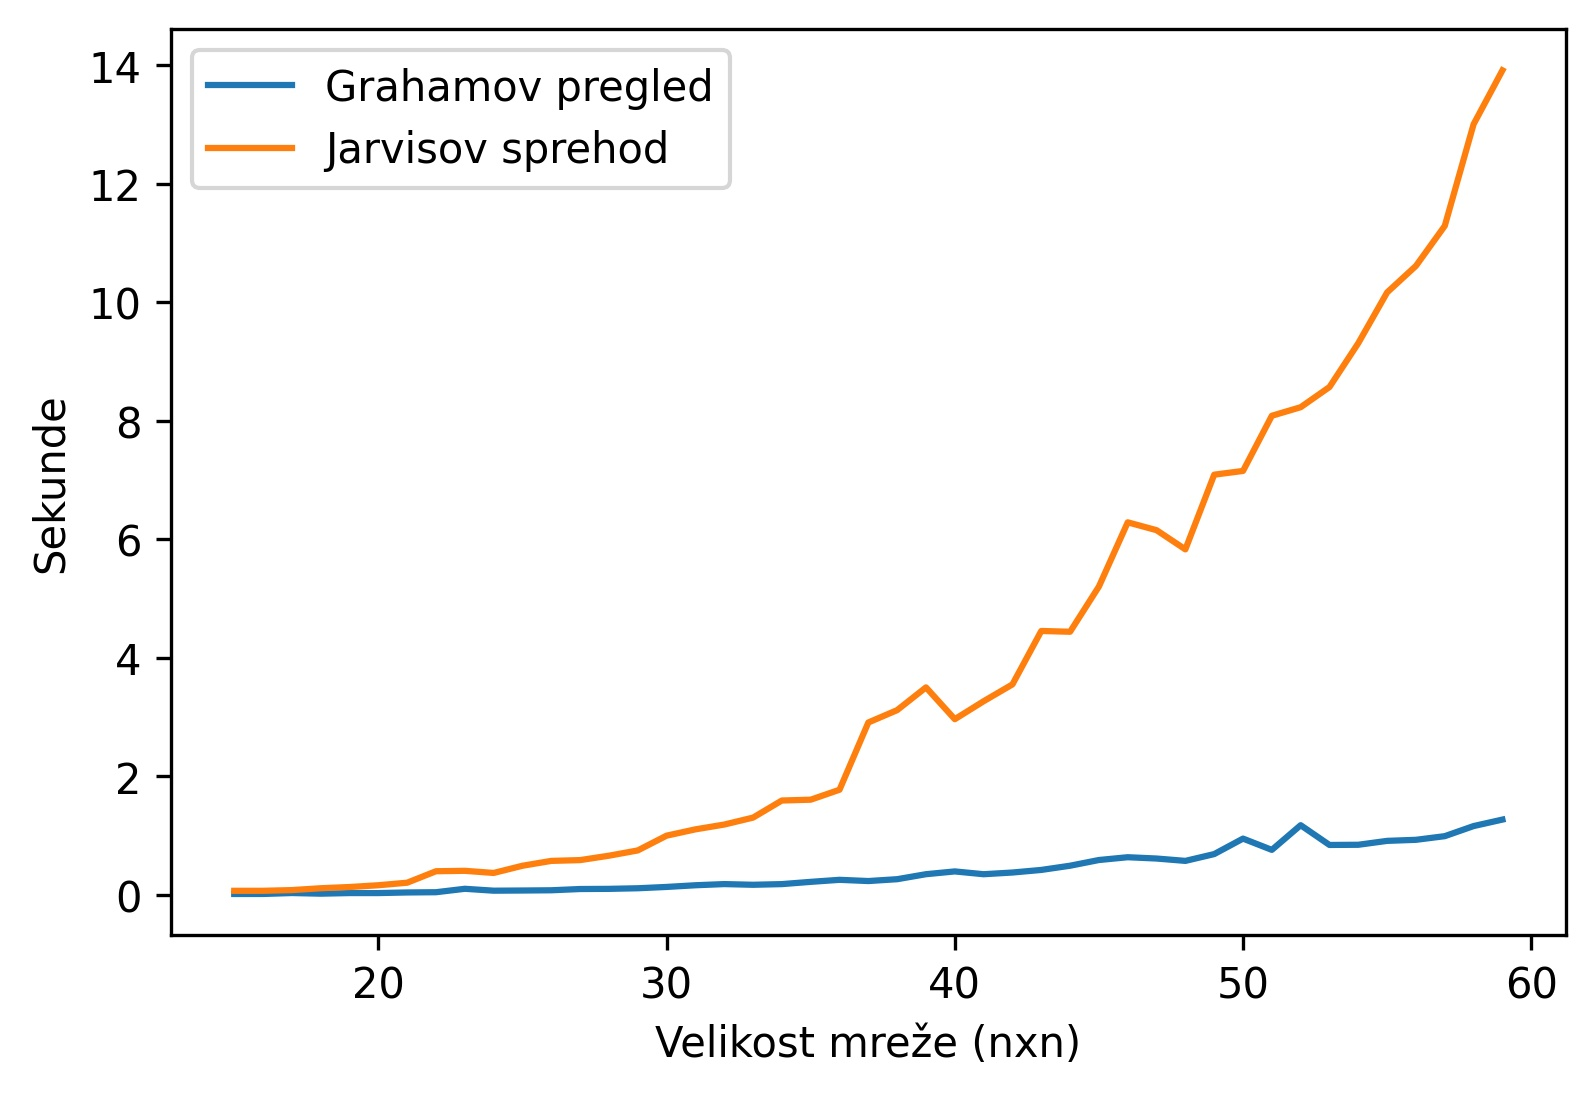
\includegraphics[scale=0.6]{slike/cas.jpg}
\end{figure}

Kot že omenjeno, je v literaturi omenjena časovna zahtevnost $O(n ^ \frac{4}{3}),$~kar pomeni, da je število konveksnih ovojnic na $n \times n$~mreži $\Theta(n ^ \frac{4}{3})$.
Na sliki \ref{fig:st_ovojnic} je predstavljeno število ovojnic izvedenega algoritma v odvisnosti od $n,$~kjer za $n$ vzamemo naravna števila od $1$ do $35$ in mreže različnih vrst. 
Opazimo, da se razmerju med številom ovojnic in velikostjo navadne mreže najbolj prilega funkcija $1,5 \cdot n ^ \frac{4}{3}.$ Eksperimentalni rezultat se torej ujema s tistim, navedenim v 
literaturi. Za potenčne $n \times n$ mreže je najboljša funkcija, ki prikaže razmerje med številom konveksnih ovojnic in velikostjo mreže, $2,3 \cdot n$, torej je časovna zahtevnost algoritma
v tem primeru $O(n)$. Na enak način za Cantorjevo $n \times n$ mrežo dobimo časovno zahtevnost $O(n^2)$, vendar pa to velja samo za $n$ manjši od 35, za višje $n$ pa se
število ovojnic Cantorjeve mreže obnaša precej nenavadno, česar pa nisva znala pojasniti. Ugibava, da gre za težave pri računanju zelo velikih števil (velikosti ranga $3^{40} \approx 10^{20}$).

\begin{figure}[!h]
	\centering
	\caption{Število ovojnic različnih $n \times n$ mrež v odvisnosti od $n$}
	\label{fig:st_ovojnic}
	\vspace{2mm}
	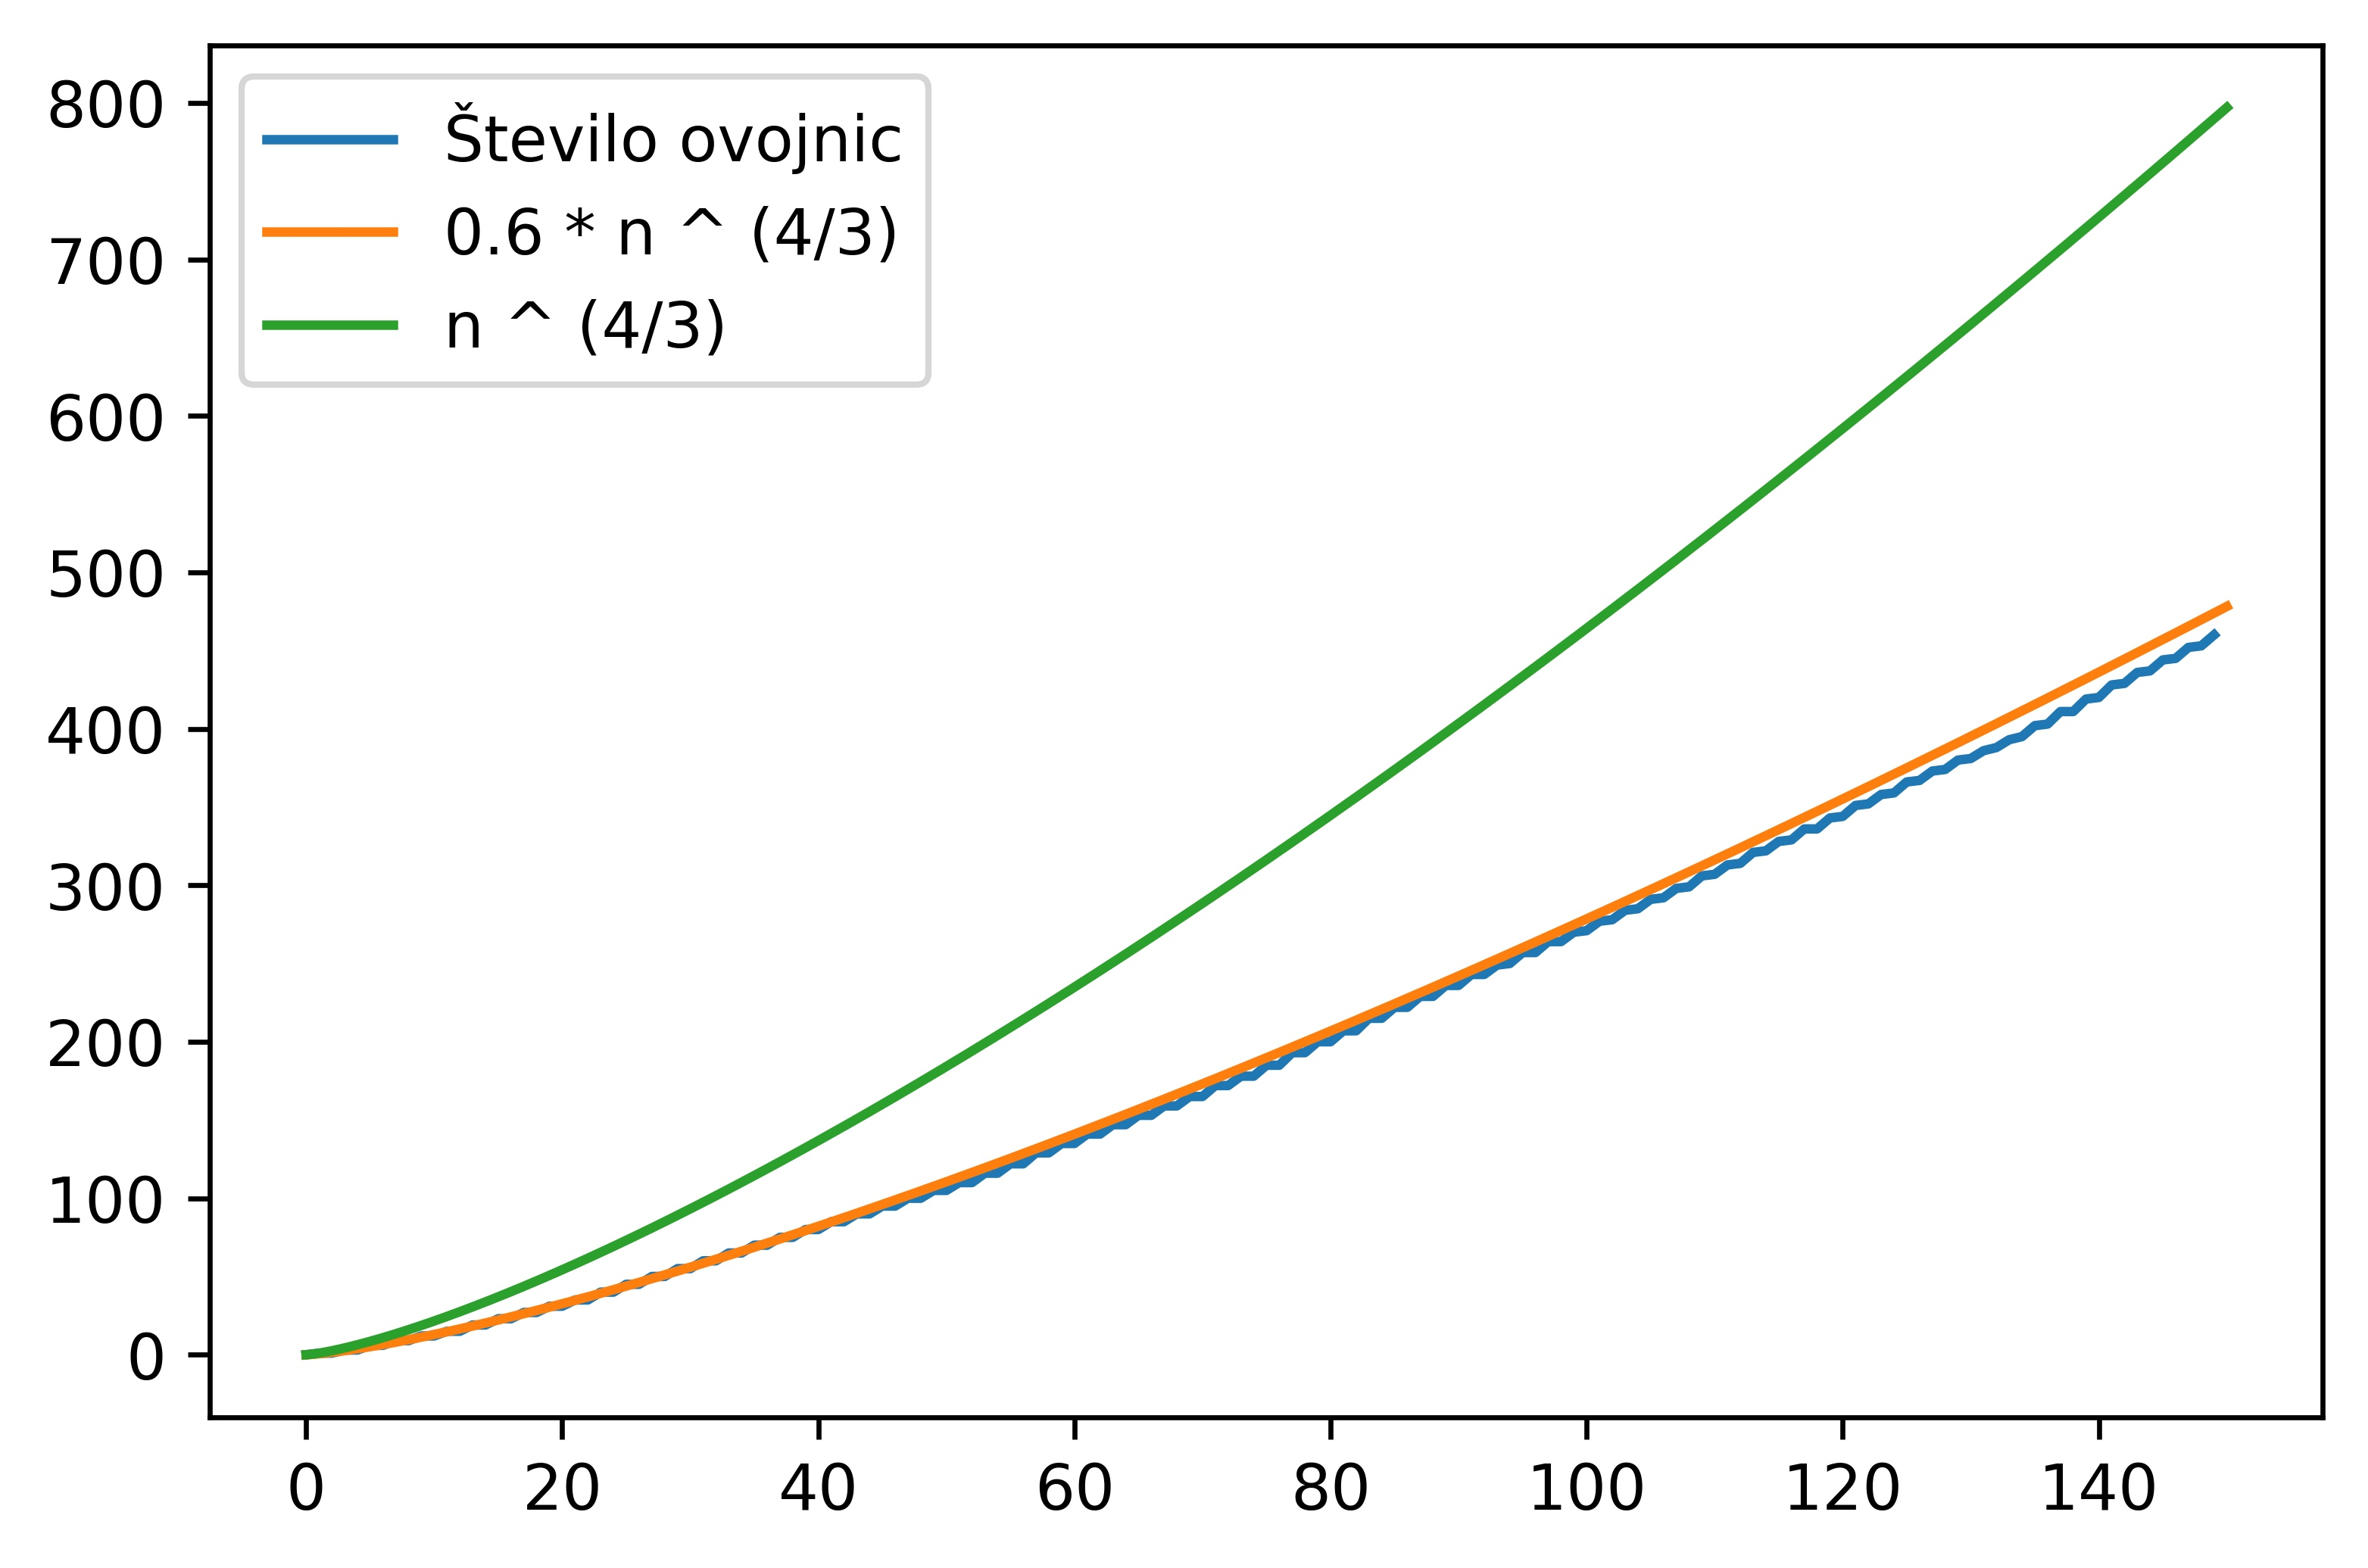
\includegraphics[scale=0.6]{slike/st_ovojnic.jpg}
\end{figure}

Za $m \times n$ mreže v literaturi ni omenjene časovne zahtevnosti, zato sva jo poiskušala določiti sama. Število ovojnic je tu odvisno od dveh parametrov, $m$ in $n$, zato je ta graf 
tridimenzionalen. Rezultate lahko vidimo na sliki \ref{fig:3d}.

\begin{figure}[!h]
	\centering
	\caption{Število ovojnic $50 \times 50$ mreže v odvisnosti od $m$ in $n$}
	\label{fig:3d}
	\vspace{2mm}
	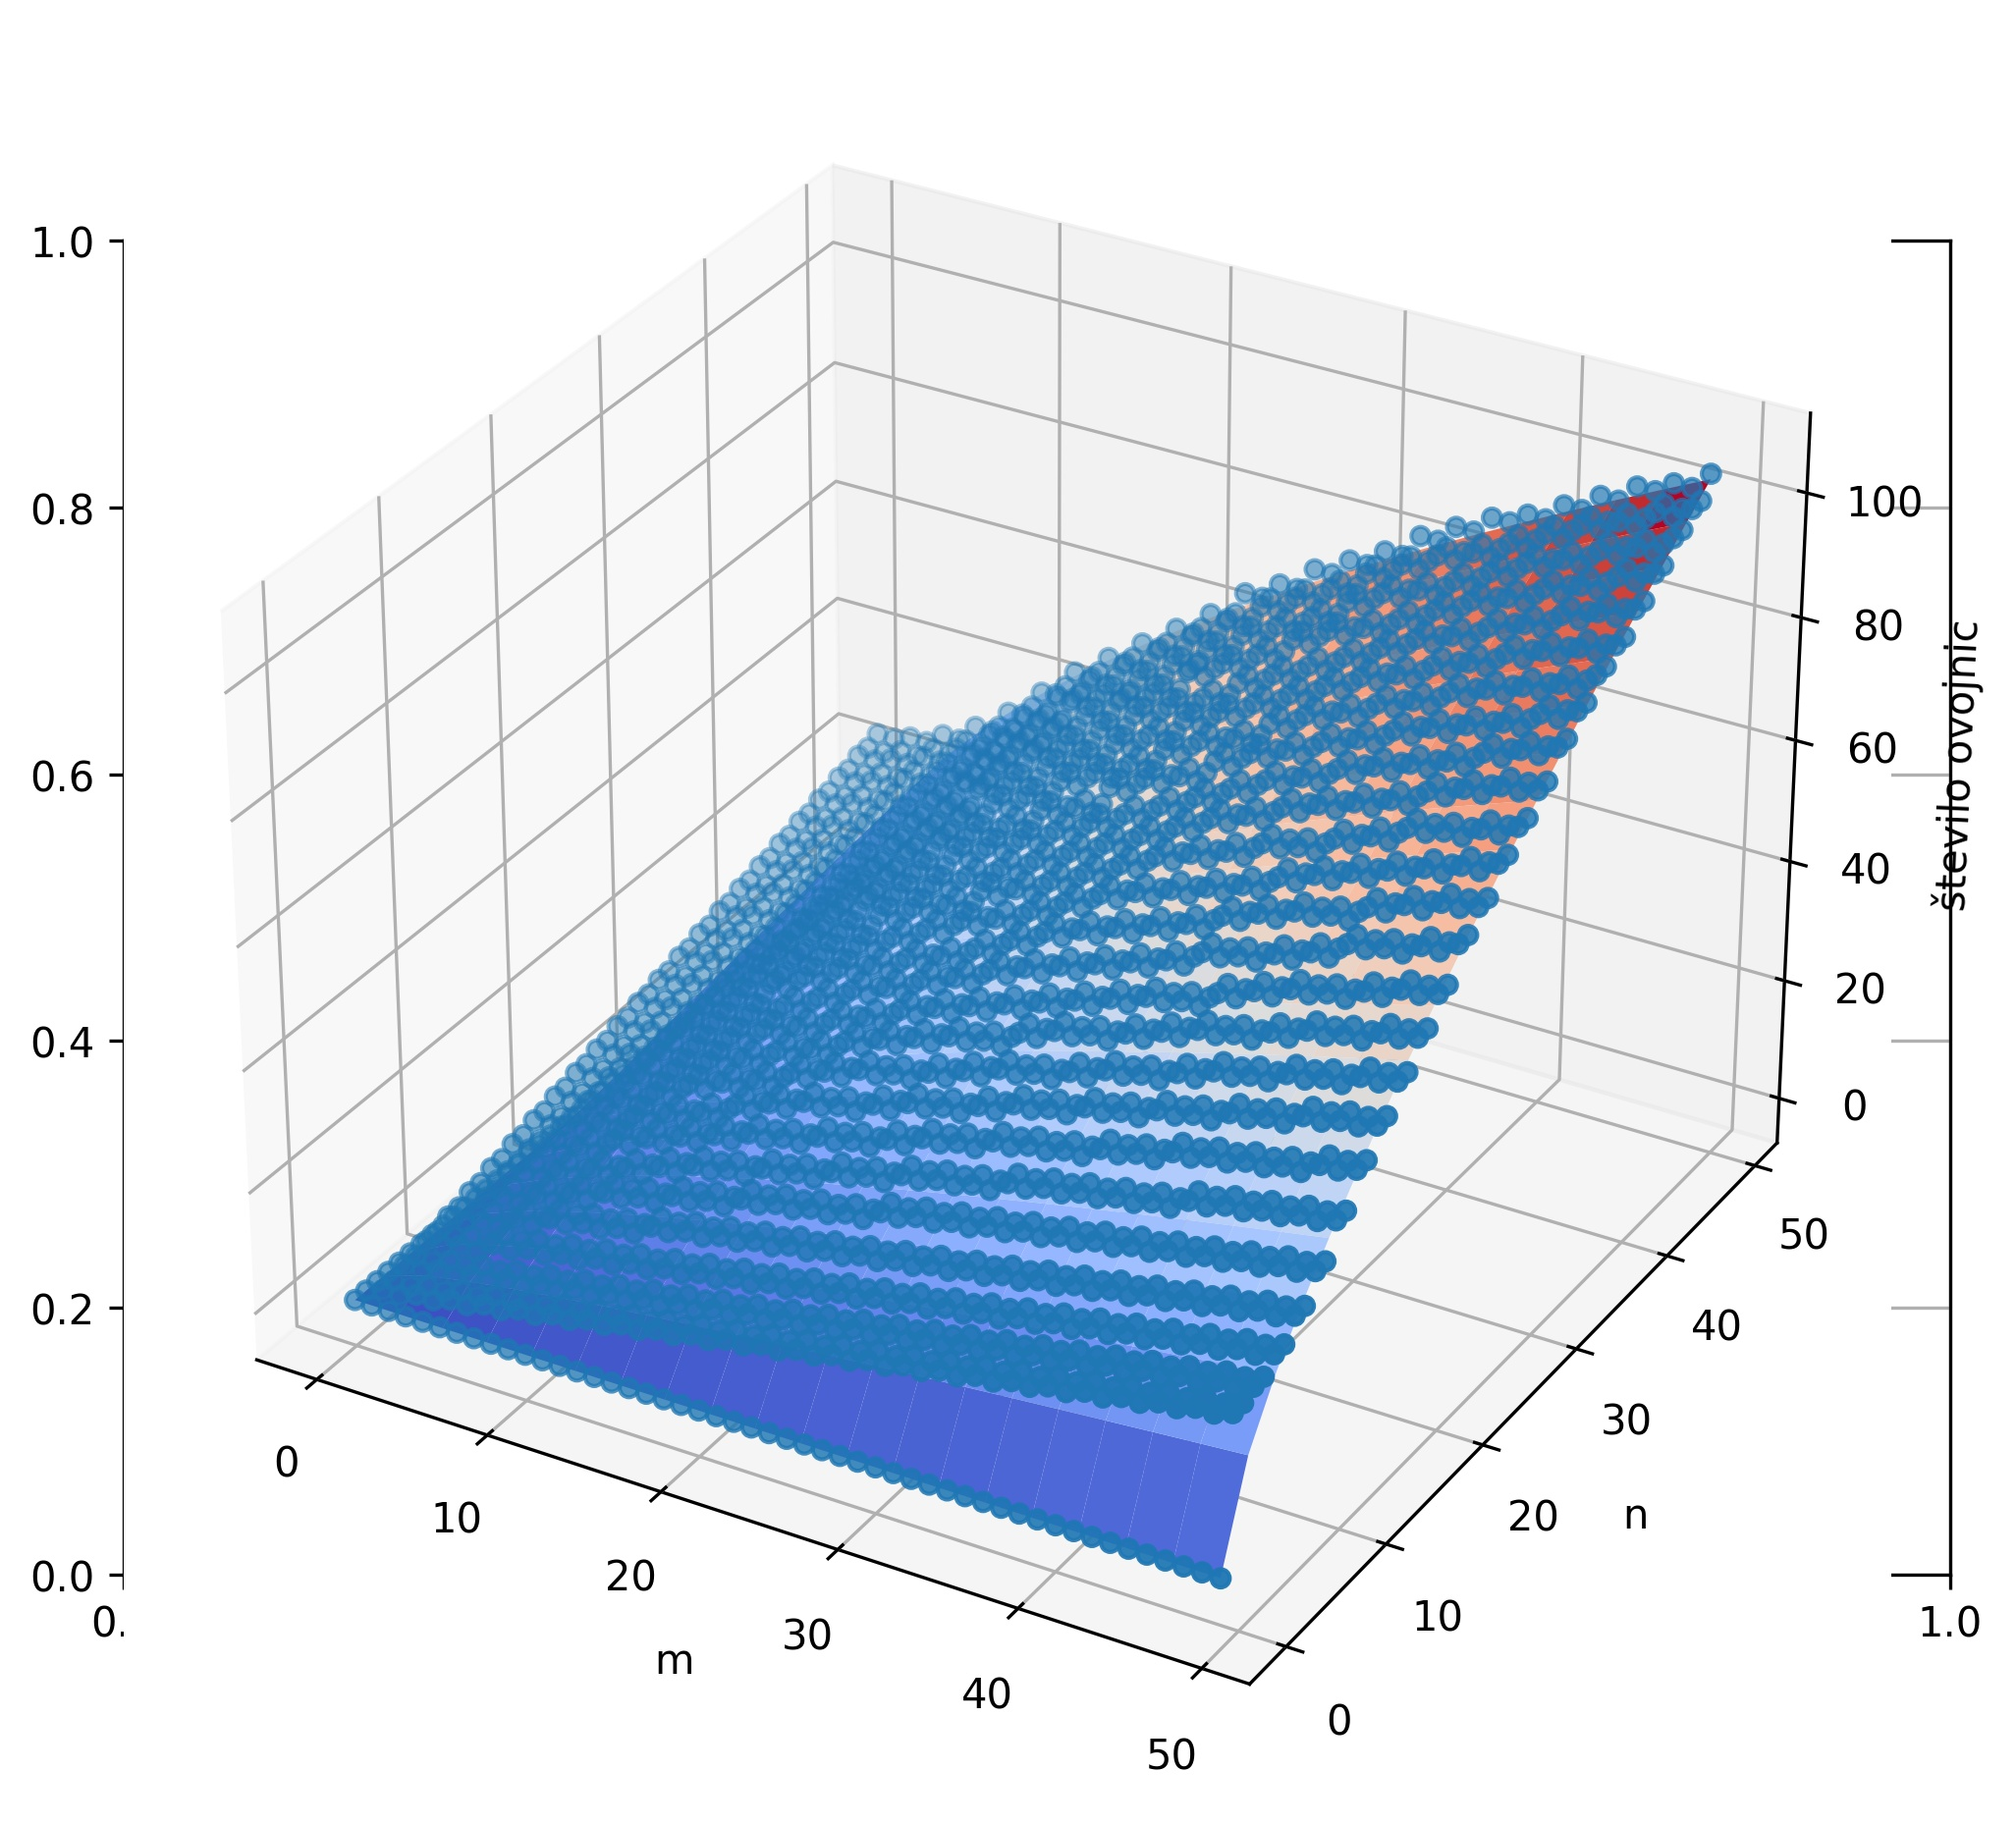
\includegraphics[scale=0.4]{slike/mxn_3d.jpg}
\end{figure}

Na zgornji sliki vidimo graf števila ovojnic mreže velikosti $50 \times 50$ v odvisnosti od $m$ in $n$. Rezultatom sva s pomočjo aproksimacijskega algoritma narisala ploskev, ki se najbolje
prilega rezultatom. Ta algoritem je sprejel podatke o številu ovojnic pri posameznih parih $(m, n)$ in narisal te točke ter ploskev oblike $a(m^b \cdot n^c)$, ki se jim najbolje prilega.
Poleg tega je vrnil še pripadajoče parametre $a, b$ in $c$ te ploskve, iz katerih sva ocenila, da je časovna zahtevnost lupljenja konveksnih ovojnic na $m \times n$ mreži 
$O((mn)^{\frac{2}{3}})$. Aproksimacijski algoritem, ki sva ga uporabila, je podrobneje predstavljen na spletni strani \cite{aproksimacija}.

\section{Rezultati}
Kot že rečeno, se za enakomerne $n \times n$ mreže, za katere je bila v literaturi podana časovna zahtevnost, teoretični in eksperimentalni podatki ujemajo. Časovna zahtevnost izvedbe algoritma
je v tem primeru torej $O(n ^ \frac{4}{3})$. Za potenčne mreže velikosti $n \times n$, tj. množice točk oblike $(2^i, 2^i), 0 \leq i \leq n - 1$, je časovna zahtevnost enaka
$O(n)$, za Cantorjeve mreže pa $O(n^2)$ (za $n \leq 35$), kar se ravno tako ujema z literaturo.
Za mreže velikosti $m \times n$ v literaturi ni bilo podatka o časovni zahtevnosti, zato sva jo določila eksperimentalno. Profesor Cabello je predvideval,
da se bo mreža obnašala podobno kot $min\{m,n\}\times min\{m,n\}$, eksperimentalno
pa sva ocenila, da je za take mreže časovna zahtevnost algoritma $O((mn)^{\frac{2}{3}})$. 

\begin{thebibliography}{3}
    \bibitem{dolg}
    David Eppstein, Sariel Har-Peled, Gabriel Nivasch. \textit{Grid Peeling and the Affine Curve-Shortening Flow}.
    \bibitem{kratek}
    Sariel Har-Peled, Bernard Lidický. \textit{Peeling the Grid}. 2012.
    \bibitem{aproksimacija}
    Fitting 3d Data, \\\href{https://stackoverflow.com/questions/53506257/fitting-3d-data?noredirect=1&lq=1}
    {\texttt{https://stackoverflow.com/questions/53506257/fitting-3d-data?noredirect=1\&lq=1}}
\end{thebibliography}

\end{document}